\section{Fysiologiske konsekvenser}\label{sec:fysio}
%I forhistorien, da mennesket var jægere, var der en naturlig favorisering af de mennesker, som kunne lagre fedt bedre end andre, da der kunne gå lang tid imellem måltiderne, hvilket ikke er nødvendigt med den moderne livsstil, hvor teknologi og højere velstand har medført et mere fysisk inaktivt liv samtidig med der er let adgang til føde. Idet evolutionen ikke har tilpasset sig denne moderne livsstil, søger kroppen stadig at lagre fedt, hvorved personer med et lavere aktivitetsniveau end den energi de indtager, langsomt vil ophobe fedtdepoter, hvilket kan resultere i overvægt.\citep{Ahmad2014,Kiens2007}

\subsection{Fysiske konsekvenser ved inaktivitet og overvægt}
\textbf{Vi vil sørge for, at dette afsnit fokuserer lidt mere på at man kan både være aktiv men også overvægtig. Desuden vil vi gå lidt mere i dybden med de fysiologiske konsekvenser af at være inaktiv og overvægtig.}
Det er veldokumenteret, at der sker et fald i fysisk aktivitet med alderen samtidig med der sker en stigning i vægt\citep{Kaprio2008}. Undersøgelser tyder på, at hvis kroppens cellulære vedligeholdelse styrkes med fysisk aktivitet, så kan aldringsprocessen nedsættes\citep{Knight2012}. Fysisk inaktivitet forstærker altså den generelle aldring og anses som værende mindst lige så farligt som overvægt. De to fænomener forekommer dog ofte samtidig, da inaktivitet kan forsage overvægt, men fysisk inaktivitet har en selvstændig helbredsmæssig betydning ligesom overvægt har. Det er muligt at være overvægtig men samtidig have en aktiv livsstil.\citep{Kaprio2008,Kiens2007,Hjort1997}

Fysisk inaktivitet kan lede til flere af de store folkesygdomme som hjertekarsygdomme, diabetes, osteoporose og psykiske lidelser. Menneskekroppen er ikke skabt til at være inaktiv, og derfor vil kroppen reagere kraftigt på det. For eksempel kan kroppen påbegynde nedbrydelse af knoglerne indefra, så de ikke vejer ret meget. 60 til 85\%\fxnote{Find nogle danske tal istedet} af verdensbefolkningen lever en stillesiddende livsstil, hvilket forstærker forekomsten af disse folkesygdomme.\citep{Kiens2007,Reshma2002,Martini2012} Derudover kan inaktivitet lede til disuse syndromet, som blandt andet indebærer svækket hud integritet, ændret respiratorisk funktion og nedsætning af sanserne\citep{Knight2012,Mosby2009}. \\
Definitionen for overvægt er globalt sat ud fra et body mass index (BMI), hvilket er forholdet mellem en persons vægt og højde. Et BMI på 25 eller derover er defineret som værende overvægt.\citep{Academic2016} \fxnote{Men er BMI egentlig den bedste metode? Tager udgangspunkt i færdigudviklede højde, så er måske ikke bedst for man} Overvægt opstår grundlæggende fordi der indtages mere energi end der forbruges. Nogle mennesker kan lagre fedt bedre end andre, hvorfor overvægt også kan være genetisk betinget.\citep{Nestle2014}\\
Overvægt øger risikoen for højt kolesteroltal, forhøjet blodtryk og diabetes samt følgesygdomme heraf som slagtilfælde og nyresygdomme. Det er dokumenteret, at der er størst risiko for tidlig død jo yngre mennesker opnår overvægt. Det er derfor essentielt at forbedre børns aktivitet og dermed mindske risikoen for overvægt.\citep{Nestle2014} Derudover ses der, at overvægtige børn ofte lider af psykologiske og sociale problemer, hvilket kombineret med overvægten kan have en negativ indvirkning på barnets fremtid i forhold til uddannelse og socioøkonomiske status\citep{Academic2016}.

Inaktivitet kombineret med overvægt øger risikoen for diverse sygdomme, men en normalvægtig inaktiv person er i større risiko for tidlig dødsfald end en overvægt aktiv person. Ifølge et 12-års studie lavet over 334.161 europæiske deltagere så tyder det på, at dobbelt så mange vil dø af inaktivitet end overvægt.\citep{Ekelund2015} En aktiv overvægt person har derudover ikke større chance for at udvikle hjertesygdomme end normalvægtige, så længe de er trænede og dyrker motion\citep{Nichols2014}. Det tyder altså på, at inaktivitet er mere skadeligt end overvægt, hvis de sammenlignes som normalvægtig inaktiv mod overvægtig aktiv.

\subsection{Fysiske konsekvenser ved aktivitet}
\textbf{Afsnittet vil senere komme til at fremhæve hvilke åbenlyse fordele der er ved en aktiv livsstil. Derudover tilføjer vi et afsnit, som handler om hvorfor netop cykling og løb er to gode motionsformer, og som dækker den aktivitet som et skolebarn udfører.
Vi vil forsøge at finde en anden figur end den benyttede.}
Fysisk aktivitet er defineret som enhver bevægelse, hvor skeletmuskler skal kontrahere og derved forbrænde energi. Der er forskellige former for fysisk aktivitet, som har forskellige intensitetsniveauer.\citep{Academic2016a} Ifølge Sundhedsstyrelsen skal et barn i alderen 5-17 år være fysisk aktiv i mindst 60 minutter om dagen med moderat til høj intensitet. Derudover anbefales det, at børn i denne alder skal indgå i en aktivitet i 30 minutter med høj intensitet tre gange om ugen.\fxnote{Sundhedsstyrelsen2016} Hvis kroppen holdes fysisk aktiv, kan dette mindske risikoen for flere kroniske sygdomme som diabetes og hjertesygdomme. Under fysisk aktivitet frigiver kroppen hormoner, som sætter gang i forskellige processer. For eksempel dannes der mere synovialvæske, hvorved bevægelse af led faciliteres. Derudover har fysisk aktivitet flere positive effekter på for eksempel knoglers metabolisme og menneskers psyke. \citep{Academic2016a,Smith1991,Academic2016b,Cotman2007}\\
Kroppen har mange reaktioner på fysisk aktivitet, hvilket blandt andet afhænger af aktivitetens krav til kroppen\fxnote{Skal muskelgrupper fremskynde en position som ved svømning og derved være udholdende eller skal muskelgrupper løfte en vægt som ved vægtløftning og derfor være eksplosiv men knap så udholdende?} og intensiteten heraf. Ved anstrengende fysisk aktivitet overtager sympatikus størstedelen af det autonome nervesystem og sætter for eksempel fordøjelsen på pause, da fordøjelse ikke længere er førsteprioritet og al kroppens energi kan bruges til aktivering af de pågældende skeletmuskler. Hjertet slår hurtigere, hvilket gør at pulsen stiger, hvorved ilt og næringsstoffer hurtigere sendes rundt i kroppen\citep{Hjerteforeningen}. Blodkar vil spile ud, så blodet i større grad kan komme til hudoverfladen og afgive den varme, som blodet fører fra de bevægende muskler. Der sker altså en stigning i pulsen og blodtrykket, og denne stigning afhænger af den pågældende aktivitets påvirkning på kroppen.\citep{Martini2012,Stanfield2013,Berchtold2010} \\
Der findes en klar sammenhæng imellem puls og kroppens reaktion på motionen. Ifølge flere studier hænger procenten af den maksimale puls sammen med, om kroppen brænder kalorier, træner den aerobe udholdenhed, forbedrer den anaerobe tolerance eller forbedrer den cardiovaskulære ydeevne\fxnote{hvilket gør, at man kan sprinte længere / er hurtigere, fordi der kommer mere ilt rundt i kroppen}. Jo højere procent desto højere puls og hårdere fysisk træning. Denne sammenhæng inddeles i zoner som ses på \figref{fig:PA_Procentpuls}.\citep{Leyland2007,Heartratejournal2015}
\begin{figure}[H]
	\centering
	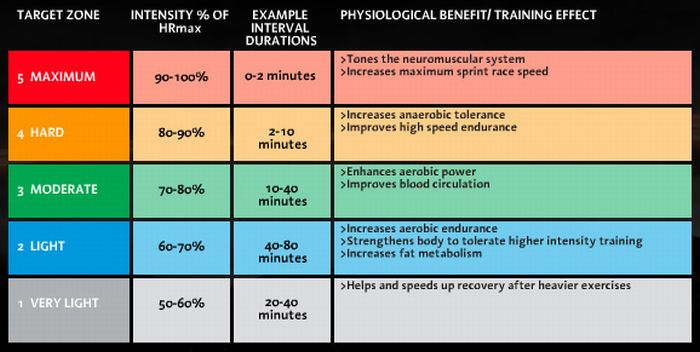
\includegraphics[scale=0.75]{figures/aProblemanalyse/heart-rate-zones.jpg}
	\caption{På figuren ses fem zoner for kroppens reaktion i forhold til pulsraten. Der ses, at de fem zoner har hver sin påvirkning på kroppen. Det er dog også anbefalet, at varigheden i hver zone bliver lavere desto hårdere aktiviteten er.\citep{Heartratejournal2015}}
	\label{fig:PA_Procentpuls}
\end{figure}
Det er dog omdiskuteret, hvorvidt zone 1 og 2 er de fortrukne, hvis ønsket er at tabe sig. Man forbrænder flere kalorier ved højintens aktivitet og derfor i zone 5. I de lavintense zoner forbrændes kalorier fra fedtceller istedet for glykogen fra muskler, hvorfor kroppen efterfølgende vil lagre kalorier i fedtcellerne, som lider underskud. Hvis man derimod dyrker højintens arbejde, som svarer til zone 4 eller 5, vil glykogenen i musklerne forbrænde, og kalorier sendes derfor til musklerne, så de kan repareres og fortsætte arbejdet. De højintense zoner kan dog ikke opretholdes over lang tid.\fxnote{Moderat intensitet svarer til 40-59\% af den maksimale iltoptagelse, eller 40-59\% af pulsreserven (maxpuls – hvilepuls), eller 64-74\% af maxpuls eller 12-13 RPE (rate of percieved excertion, Borgskala) og er yderligere defineret som fysisk aktivitet hvor man bliver lettere forpustet men hvor samtale er mulig. \citep{Kiens2007}}
%Der findes mange versioner af \figref{fig:PA_Procentpuls}, som altså kan være misvisende.
\citep{Martini2012,Leyland2007,Heartratejournal2015} 
%
%
	% Sundhedsstyrrelsens anbefalinger, sygdomme det hjælper på, fortsat af notater.
% Opbygning af afsnit %%%%%%%%%%%%%%%%%%%%%%%%%%%%%%%%%%%%%%%%%%%%%%
%-- Inaktivt og/eller overvægtig
% Kort introduktion, beskrivelse af hh. inaktivitet og overvægt.
% Følgesygdomme fra begge
% Sammenligning (Hvad er farligst, hvad er forskellen)
%-- Aktivt
% Kort introduktion, hvad betyder det at være aktiv(definition)
% Hvilken betydning har puls for forbrænding?
% Helbred 
%-- Kongnitiv funkktion (indlæring/Koncentration)
% Inaktivitet, overvægt og aktivitets påvirkning af kongitiv funktion (I hvor lang tid kan aktivitet hjælpe på indlæring?)
% Hvornår skal man være aktiv i forhold til undervisning?